\begin{name}
	{\tenchude}
	{\tendethi}
	{\tentruong}
	{\thoigian}
\end{name}
\setcounter{ex}{0}\setcounter{bt}{0}
\TN
\begin{ex}%[Dự án TeX hóa đề cấu trúc mới 2025, Đoàn Hùng]%[1D1N1-3]
Trên đường tròn lượng giác với gốc $A(1;0)$. Điểm biểu diễn góc lượng giác có số đo nào dưới đây trùng với điểm biểu diễn góc lượng giác có số đo bằng $\dfrac{7\pi }{4}$?
\choice
{\True $-\dfrac{\pi }{4}$}
{$\dfrac{\pi }{4}$}
{$\dfrac{3\pi }{4}$}
{$-\dfrac{3\pi }{4}$}
\loigiai{
Hai số đo góc lượng giác $\alpha $ và $\beta $ có cùng điểm biểu diễn trên đường tròn lượng giác khi $\alpha -\beta =k2\pi ,k\in \mathbb{Z}$.\\
Vì $\dfrac{7\pi }{4}-\left(-\dfrac{\pi }{4}\right)=2\pi $ nên đáp án là $-\dfrac{\pi }{4}$.}
\end{ex}

\begin{ex}%[1D1H3-2]
Cho $\tan (a+b)=3$, $\tan (a-b)=2$. Tính $\tan 2a$.
\choice
{\True $-1$}
{$\dfrac{1}{2}$}
{$-\dfrac{5}{6}$}
{$\dfrac{6}{5}$}
\loigiai{
Ta có: $\tan 2a=\tan \left(a+b+a-b\right)=\dfrac{\tan (a+b)+\tan (a-b)}{1-\tan (a+b)\cdot\tan (a-b)}=\dfrac{3+2}{1-3\cdot 2}=-1$.}
\end{ex}

\begin{ex}%[1D1N4-4]
Khẳng định nào dưới đây là đúng?
\choice
{Hàm số $y=\cos x$ là hàm số lẻ}
{Hàm số $y=\cot x$ là hàm số chẵn}
{\True Hàm số $y=\sin x$ là hàm số lẻ}
{Hàm số $y=\tan x$ là hàm số chẵn}
\loigiai{
Các hàm số $y=\sin x$, $y=\tan x$, $y=\cot x$ là hàm số lẻ.\\
Hàm số $y=\cos x$ là hàm số chẵn.
}
\end{ex}

\begin{ex}%[Dự án BGK10-11,2024]%[Nguyễn Văn Nay]%[1D1H4-6][Mức độ 2]
Cho hàm số $y=-\cos\left(2x+\dfrac{\pi}{3}\right)$. Gọi $m$, $M$ lần lượt là giá trị nhỏ nhất và giá trị lớn nhất của hàm số trên $\left[-\dfrac{2\pi}{3}; \dfrac{\pi}{3}\right]$. Tích $m\cdot M$ bằng bao nhiêu?
\choice
{\True $-1$}
{$-\dfrac{1}{2}$}
{$\dfrac{1}{2}$}
{$-\dfrac{1}{4}$}
\loigiai{
Khi $x\in \left[-\dfrac{2\pi}{3};\dfrac{\pi}{3}\right]$	thì $2x+\dfrac{\pi}{3}\in \left[-\pi;\pi\right]$, do đó $-\cos\left(2x+\dfrac{\pi}{3}\right)\in \left[-1;1\right]$.\\
Vậy giá trị nhỏ nhất và giá trị lớn nhất của hàm số lần lượt là $m=-1$ và $M=1$, tích $mM=-1$.
}
\end{ex}

\begin{ex}%[1D1H4-7]%[BG K11, Nhật Thiện][Mức độ 2]
\immini{Đồ thị trong hình vẽ bên là đồ thị của hàm số nào dưới đây?
\choice
{$y=\sin 2x$}
{$y=2\cos x$}
{$y=\cos 2x$}
{\True $y=2\sin x$}
}
{\begin{tikzpicture}[scale=0.8,>=stealth, font=\footnotesize, line join=round, line cap=round]
\def\xmin{-4} \def\xmax{4} \def\ymin{-2.5} \def\ymax{2.8}
\draw[->] (\xmin,0)--(\xmax,0) node [below]{$x$};
\draw[->] (0,\ymin)--(0,\ymax) node [right]{$y$};
\node at (0,0) [below right]{$O$};
\clip (\xmin+0.1,\ymin+0.1) rectangle (\xmax-0.5,\ymax-0.1);
\draw[smooth,samples=400,domain=\xmin:\xmax] plot(\x,{2*sin(\x r)});
\draw[dashed] (\xmin,2)--(\xmax,2) (\xmin,-2)--(\xmax,-2);
\foreach \x in {-2*pi,-1.5*pi,-pi,-0.5*pi,0}
{\draw[fill=black] (\x,2*sin \x*180/pi) circle (1pt);
\draw[dashed] (\x,2*sin \x*180/pi)--(\x,0);
\draw[fill=black] (-\x,2*sin -\x*180/pi) circle (1pt);
\draw[dashed] (-\x,2*sin -\x*180/pi)--(-\x,0);}
\node at (0,2.3) [left]{$2$};
\node at (0,-2.3) [left]{$-2$};
\node at (-2*pi+0.15,0) [below]{$-2\pi$};
\node at (-1.5*pi,0) [below]{$-\frac{3\pi}{2}$};
\node at (-pi-0.15,0) [below]{$-\pi$};
\node at (-0.5*pi,0) [above]{$-\frac{\pi}{2}$};
\node at (0.5*pi,0) [below]{$\frac{\pi}{2}$};
\node at (pi-0.1,0) [below]{$\pi$};
\node at (1.5*pi,0) [above]{$\frac{3\pi}{2}$};
\node at (2*pi+0.2,0) [below]{$2\pi$};
\end{tikzpicture}}
\loigiai{
Từ đồ thị ta thấy hàm số đi qua gốc tọa độ $O(0;0)$, có tung độ cao nhất bằng $2$ và thấp nhất bằng $-2$. Chỉ có hàm số $y=2\sin x$ thỏa mãn.}
\end{ex}

\begin{ex}%[De-chuan-hoa-so-15]%[Trần Văn Hùng]%[1D1N5-1]
Trong các khẳng định sau khẳng định nào đúng?
\choice
{Phương trình $\sin x =a$ có nghiệm với mọi số thực $a$}
{\True Phương trình $\tan x =a$ và phương trình $\cot x =a$ có nghiệm với mọi số thực $a$}
{Phương trình $\cos x =a$ có nghiệm với mọi số thực $a$}
{Phương trình $\tan x =a$ và phương trình $\cot x =a$ vô nghiệm khi $a>1$}
\loigiai{
Phương trình $\tan x =a$ và phương trình $\cot x =a$ có nghiệm với mọi số thực $a$.
}
\end{ex}

\begin{ex}%[1D2N1-4]%[1D2N1-5]
Cho dãy số $(a_n)$ có $a_n=\dfrac{5}{2^n}$. Tính chất nào sau đây của dãy số $(a_n)$ là đúng?
\choice
{Tăng và không bị chặn}
{\True Giảm và bị chặn dưới}
{Tăng và bị chặn trên}
{\True Giảm và bị chặn trên}
\loigiai{
Ta có \\
$a_{n+1}=\dfrac{5}{2^{n+1}}=\dfrac{5}{2^n\cdot 2}<\dfrac{5}{2^n}=a_n$, $\forall n\in \mathbb{N^*}$\\
$a_n=\dfrac{5}{2^n}\leq \dfrac{5}{2}$, $\forall n\in \mathbb{N^*}$\\
$a_n=\dfrac{5}{2^n}>0$, $\forall n\in \mathbb{N^*}$\\
Vậy dãy số $(a_n)$ là dãy số giảm và bị chặn.
}
\end{ex}

\begin{ex}%[De-chuan-hoa-so-25]%[Phạm Ngọc Trung]%[1D2N1-3]
Cho dãy số $\left(u_n\right)$ với $\heva{& u_1=1\\ & u_{n+1}=u_n+n^2\,, n \ge 1}$. Số hạng thứ $2$ của dãy số là số hạng nào dưới đây?
\choice
{$u_2=5$}
{$u_2=7$}
{\True $u_2=2$}
{$u_2=1$}
\loigiai{
Ta có $u_2=u_1+1^2=1+1=2$.
}
\end{ex}

\begin{ex}%[1D2H2-3]
Cho dãy số $(u_n)$ xác định bởi: $u_1=3$ và  $u_n = u_{n-1}+5$ với mọi $n \ge 2.$ Tìm công thức của số hạng tổng quát $u_n.$
\choice
{$u_n = n-2$}
{$u_n = -5n-2$}
{\True $u_n = 5n-2$}
{$u_n = 5n+2$}
\loigiai{
Ta có $u_n-u_{n-1}=5$ nên dãy $(u_n)$ là cấp số cộng với công sai $d=5$ và số hạng đầu $u_1=3$. \\
Do đó, $u_n=5n-2$.
}
\end{ex}

\begin{ex}%[12EX-OnTap-Form2025-Nguyễn Đắc Giáp]%[1D2H2-6]
Cho $\left(u_n\right)$ là cấp số cộng có $u_2+u_9=15$. Tổng 10 số hạng đầu tiên của cấp số cộng đó bằng
\choice
{$150$}
{\True $75$}
{$120$}
{$90$}
\loigiai{
Ta có \[u_2+u_9=15\Leftrightarrow (u_1+d)+(u_1+8d)=15\Leftrightarrow 2u_1+9d=15.\]
Suy ra
\[ S_{10}=\dfrac{10}{2}\left(2u_1+9d\right) = 5 \cdot 15 =75.\]

}
\end{ex}

\begin{ex}%[1D2N3-2]
Trong các dãy số sau, dãy số nào là cấp số nhân?
\choice
{$-3; 1; 5; 9; \ldots$}
{$\dfrac{1}{2}; \dfrac{2}{3}; \dfrac{3}{4}; \dfrac{4}{5}; \ldots$}
{\True $16; 8; 4; 2; \ldots$}
{$3; 6; 18; 108; \ldots$}
\loigiai{
\begin{itemize}
\item Dãy số $-3; 1; 5; 9; \ldots$ không là CSN vì $\dfrac{1}{-3}\neq \dfrac{5}{1}$.
\item Dãy số $\dfrac{1}{2}; \dfrac{2}{3}; \dfrac{3}{4}; \dfrac{4}{5}; \ldots$ không là CSN vì $\dfrac{2}{3}: \dfrac{1}{2}\neq \dfrac{3}{4}: \dfrac{2}{3}$.
\item Dãy số $16; 8; 4; 2; \ldots$ là CSN vì $\forall n\in \mathbb{N}^*$ ta có $u_{n+1}=u_n\cdot q$.
\item Dãy số $3; 6; 18; 108; \ldots$ không là CSN vì $\dfrac{6}{3}\neq \dfrac{18}{6}$.
\end{itemize}
}
\end{ex}

\begin{ex}%[1D2H3-3]%[Dự án 11 HVA 2024-2025]%[Võ NGuyên Thạch]
Cho cấp số nhân $\left(u_n\right)$ có $u_3=12$, $u_5=48$, có công bội âm. Tổng $7$ số hạng đầu của cấp số nhân đã cho bằng
\choice
{\True $129$}
{$-129$}
{$128$}
{$-128$}
\loigiai{
Ta có $u_4^2=u_3\cdot u_5=576$.\\
Vì $u_3>0$, $u_5>0$ và công bội âm nên $u_4=-24\Rightarrow q=-2$.\\
Lại có $u_3=u_1q^2\Rightarrow u_1=\dfrac{u_3}{q^2}=\dfrac{12}{4}=3$.\\
Áp dụng công thức ta có $S_7=u_1\dfrac{1-q^7}{1-q}=3\cdot \dfrac{1-\left(-2\right)^7}{1-\left(-2\right)}=129$.
}
\end{ex}

\begin{ex}%[Dự án 11 HVA 2024-2025]%[Trần Nam Nhất]%[1D5H1-2]
Mức thưởng tết cho các nhân viên của một công ty được thống kê trong bảng sau
\begin{center}
\begin{tabular}{|c|c|c|c|c|c|}
\hline
Mức thưởng tết & $[5;10)$ & $[10;15)$ & $[15;20)$ & $[20;25)$ & $[25;30)$ \\
\hline
Số nhân viên & $13$ & $35$ & $47$ & $25$ & $10$ \\
\hline
\end{tabular}
\end{center}
Giá trị đại diện của nhóm $[15;20)$ là
\choice
{$5$}
{\True $17{,}5$}
{$30$}
{$130$}
\loigiai{
Giá trị đại diện của nhóm $[15;20)$ là $\dfrac{15+20}{2}=17{,}5$.
}
\end{ex}

\begin{ex}%[1D5H1-3]
Bạn Chi rất thích nhảy hiện đại. Thời gian tập nhảy mỗi ngày trong thời gian gần đây của bạn Chi được thống kê lại ở bảng sau
\begin{center}
\begin{tabular}{|c|c|c|c|c|c|}
\hline
Cự li (m) & $\left[19; 19{,}5\right)$ & $\left[19{,}5; 20\right)$ & $\left[20; 20{,}5\right)$ & $\left[20{,}5; 21\right)$ & $\left[21; 21{,}5\right)$ \\
\hline
Tần số & $13$ & $45$ & $24$ & $12$ & $6$ \\
\hline
\end{tabular}
\end{center}
Số trung bình của mẫu số liệu ghép nhóm là
\choice
{$100$}
{\True $20{,}015$}
{$2001{,}5$}
{$2$}
\loigiai{
Cỡ mẫu $n=100$.
\begin{center}
\begin{tabular}{|c|c|c|c|c|c|}
\hline
Cự li (m) & $\left[19; 19{,}5\right)$ & $\left[19{,}5; 20\right)$ & $\left[20; 20{,}5\right)$ & $\left[20{,}5; 21\right)$ & $\left[21; 21{,}5\right)$ \\
\hline
Giá trị đại diện & $19{,}25$ & $19{,}75$ & $20{,}25$ & $20{,}75$ & $21{,}25$ \\
\hline
Tần số & $13$ & $45$ & $24$ & $12$ & $6$ \\
\hline
\end{tabular}
\end{center}
Số trung bình của mẫu số liệu ghép nhóm là
\[\bar{x}= \dfrac{19{,}2\cdot 13+19{,}75\cdot 45+20{,}25\cdot 24+20{,}75\cdot 12+21{,}25\cdot 6}{100}=20{,}015 .\]
}
\end{ex}

\begin{ex}%[Dự án 11 HVA 2024-2025]%[Chu Hà]%[1D5H2-2]
Cân nặng của các em học sinh nam lớp $11A$ được thống kê ở bảng sau
\begin{center}
\begin{tabular}{|c|c|c|c|c|c|c|}
\hline
Cân nặng & $[45;49)$ & $[49;53)$ & $[53;57)$ & $[57;61)$ & $[61;65)$ \\
\hline
Số học sinh & $4$ & $5$ & $7$ & $7$ & $5$ \\
\hline
\end{tabular}

\end{center}
Trung vị của mẫu số liệu trên là
\choice
{$55{,}85$}
{$55{,}87$}
{$53{,}86$}
{\True $55{,}86$}
\loigiai{
Gọi $x_1$, $x_2$, {\dots}, $x_{28}$ là cân nặng của các em học sinh lớp $11A$ xếp theo thứ tự không giảm.\\
Do $x_1$, $x_2$, $x_3$, $x_4 \in \left[45;49\right)$; $x_5$, $\ldots$, $x_9 \in \left[49;53\right)$; $x_{10}$, $\ldots$, $x_{16} \in \left[53;57\right)$; $x_{17}$, $\ldots$, $x_{23} \in \left[57;61\right)$; $x_{24}$, $\ldots$, $x_{28} \in \left[61;65\right)$ nên trung vị của mẫu số liệu $x_1$, $x_2$, $\ldots$, $x_{28}$ là $\dfrac{1}{2} \left(x_{14}+x_{15} \right)\in \left[53;57\right)$.\\
Ta xác định được $n=28$, $n_m=7$, $C=4+5=9$, $u_m=53$, $u_{m+1}=57$. Vậy trung vị của mẫu số liệu ghép nhóm là
\[M_e=53+\dfrac{\dfrac{28}{2}-9}{7} \left(57-53\right)\approx 55{,}86.\]
}
\end{ex}

\begin{ex}%[1H4H1-1]
Trong không gian, cho hai đường thẳng $a$, $b$ và mặt phẳng $\left( P \right)$. Mệnh đề nào đúng?
\choice
{Nếu $a$ nằm trong $\left( P \right)$ và $a$ cắt $b$ thì $b$ nằm trong $\left( P \right)$}
{Nếu $a$ chỉ chứa một điểm chung với $\left( P \right)$ thì $a$ nằm trong $\left( P \right)$}
{\True Nếu $b$ chứa hai điểm phân biệt thuộc $\left( P \right)$ thì $b$ nằm trong $\left( P \right)$}
{Nếu $a$ và $b$ cùng nằm trong $\left( P \right)$ thì $a$ cắt $b$}
\loigiai{}
\end{ex}

\begin{ex}%[1H4N1-2]
Cho hình chóp $S.ABCD$ có đáy $ABCD$ là hình thang, đáy lớn $AB$ gấp đôi đáy nhỏ $CD$, $E$ là trung điểm của đoạn $AB$. Hình vẽ nào sau đây đúng quy tắc?
\choice
{\begin{tikzpicture}[line join = round, line cap = round,font=\footnotesize,>=stealth,scale=1]
\coordinate (B) at (-1,1);
\coordinate (A) at (3,2);
\coordinate (C) at (0,0);
\coordinate (D) at (2,0);
\coordinate (S) at (-1,4);
\coordinate (E) at ($(A)!0.5!(B)$);
\draw (B)--(C)--(D)--(A) (C)--(S)--(B) (A)--(S)--(D);
\draw[dashed,thin](B)--(A) ;
\foreach \i/\g in {A/0,B/180,C/-90,D/-90,S/90,E/90}{\draw[fill=black](\i) circle (1pt) ($(\i)+(\g:3mm)$) node[scale=1]{$\i$};}
\end{tikzpicture}}
{\begin{tikzpicture}[line join = round, line cap = round,font=\footnotesize,>=stealth,scale=1]
\coordinate (B) at (-1,1);
\coordinate (A) at (3,1);
\coordinate (C) at (0,0);
\coordinate (D) at (2,0);
\coordinate (S) at (-1,4);
\coordinate (E) at ($(A)!0.5!(B)$);
\draw (A)--(B)--(C)--(D)--(A) (C)--(S)--(B) (A)--(S)--(D);
\foreach \i/\g in {A/0,B/180,C/-90,D/-90,S/90,E/90}{\draw[fill=black](\i) circle (1pt) ($(\i)+(\g:3mm)$) node[scale=1]{$\i$};}
\end{tikzpicture}}
{\True \begin{tikzpicture}[line join = round, line cap = round,font=\footnotesize,>=stealth,scale=1]
\coordinate (B) at (-1,1);
\coordinate (A) at (3,1);
\coordinate (C) at (0,0);
\coordinate (D) at (2,0);
\coordinate (S) at (-1,4);
\coordinate (E) at ($(A)!0.5!(B)$);
\draw (B)--(C)--(D)--(A) (C)--(S)--(B) (A)--(S)--(D);
\draw[dashed,thin](B)--(A) ;
\foreach \i/\g in {A/0,B/180,C/-90,D/-90,S/90,E/-90}{\draw[fill=black](\i) circle (1pt) ($(\i)+(\g:3mm)$) node[scale=1]{$\i$};}
\end{tikzpicture}}
{\begin{tikzpicture}[line join = round, line cap = round,font=\footnotesize,>=stealth,scale=1]
\coordinate (B) at (-1,1);
\coordinate (A) at (3,1);
\coordinate (C) at (0,0);
\coordinate (D) at (2,0);
\coordinate (S) at (-1,4);
\coordinate (E) at ($(B)!0.7!(A)$);
\draw (B)--(C)--(D)--(A) (C)--(S)--(B) (A)--(S)--(D);
\draw[dashed,thin](B)--(A) ;
\foreach \i/\g in {A/0,B/180,C/-90,D/-90,S/90,E/90}{\draw[fill=black](\i) circle (1pt) ($(\i)+(\g:3mm)$) node[scale=1]{$\i$};}
\end{tikzpicture}}
\loigiai{
Hình vẽ đúng qui tắc là hình vẽ sau:
\begin{center}
\begin{tikzpicture}[line join = round, line cap = round,font=\footnotesize,>=stealth,scale=1]
\coordinate (B) at (-1,1);
\coordinate (A) at (3,1);
\coordinate (C) at (0,0);
\coordinate (D) at (2,0);
\coordinate (S) at (-1,4);
\coordinate (E) at ($(A)!0.5!(B)$);
\draw (B)--(C)--(D)--(A) (C)--(S)--(B) (A)--(S)--(D);
\draw[dashed,thin](B)--(A) ;
\foreach \i/\g in {A/0,B/180,C/-90,D/-90,S/90,E/-90}{\draw[fill=black](\i) circle (1pt) ($(\i)+(\g:3mm)$) node[scale=1]{$\i$};}
\end{tikzpicture}
\end{center}
}
\end{ex}

\begin{ex}%[1H4H1-3]
\immini{Cho hình chóp $S.ABCD$ có đáy là hình thang với đáy lớn $AB$. Gọi $M$ là trung điểm $SC$. Tìm giao tuyến của mặt phẳng $(MAD)$ và $(SBC)$.
\choice
{$ME$ (với $E$ là giao điểm của $AB$ và $CD$)}
{\True $ME$ (với $E$ là giao điểm của $AD$ và $BC$)}
{$SE$ (với $E$ là giao điểm của $AB$ và $CD$)}
{ $SE$ (với $E$ là giao điểm của $AD$ và $BC$)}}{
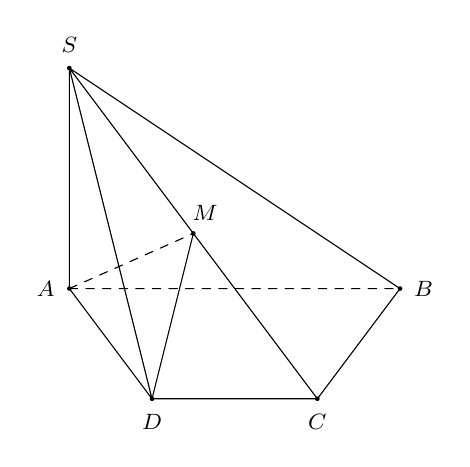
\begin{tikzpicture}[scale=0.7, font=\footnotesize, line join=round, line cap=round, >=stealth]
\path (0,0)coordinate(A)
--++(1.5,-2) coordinate(D)
--++(3,0) coordinate(C)
(A)--+(6,0) coordinate (B)
--+(0,4) coordinate (S)
(S)--(C) coordinate[pos=0.5](M);
\draw (S)--(D)--(C)--(B)--cycle (S)--(C) (S)--(A) (A)--(D)--(M);
\draw[dashed] (A)--(B) (A)--(M);
\foreach \p/\q in {A/180,D/-90,C/-90,B/0,S/90,M/60}{
\path (\p) node[shift={(\q:3mm)}]{$\p$};
\fill[black] (\p) circle (1.2pt);}
\end{tikzpicture} }
\loigiai{
\immini{Ta có $M\in (MAD)$.\\
Mặt khác $M\in SC$, $SC\subset (SBC) \Rightarrow M\in (SBC)$ nên $M$ là điểm chung thứ nhất của hai mặt phẳng $(SBC)$ và $(MAD)$.\\
Trong mặt phẳng $(ABCD)$ gọi $E = AD \cap BC$\\
$\Rightarrow \heva{& E\in AD \\& E \in BC}\Rightarrow \heva{& E \in (MAD) \\& E \in (SBC)}\Rightarrow E\in (MAD)\cap (SBC)$.\\
Vậy $ME= (MAD)\cap (SBC)$.}{
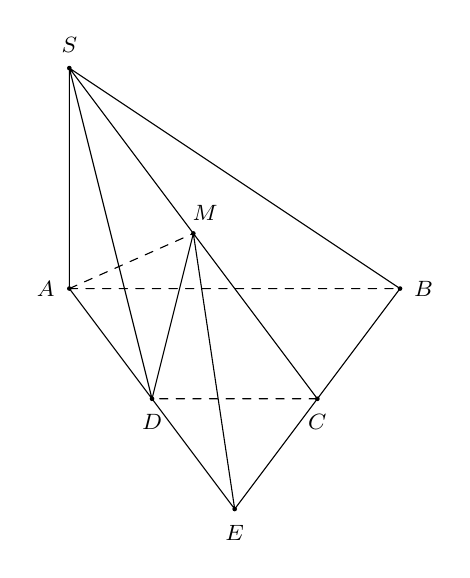
\begin{tikzpicture}[scale=0.7, font=\footnotesize, line join=round, line cap=round, >=stealth]
\path (0,0)coordinate(A)
--++(1.5,-2) coordinate(D)
--++(3,0) coordinate(C)
(A)--+(6,0) coordinate (B)
--+(0,4) coordinate (S)
(S)--(C) coordinate[pos=0.5](M)
(intersection of A--D and B--C) coordinate(E)
;
\draw (D)--(S) --(B)--(C) (S)--(C) (S)--(A) (A)--(D) (D)--(E)--(C) (D)--(M)--(E);
\draw[dashed] (A)--(B) (A)--(M) (C)--(D) ;
\foreach \p/\q in {A/180,D/-90,C/-90,B/0,S/90,M/60,E/-90}{
\path (\p) node[shift={(\q:3mm)}]{$\p$};
\fill[black] (\p) circle (1.2pt);}
\end{tikzpicture}
}
}
\end{ex}

\begin{ex}%[1H4H1-4]%[Dự án 2025 - Đề cấu trúc mới của Bộ theo
Cho hình chóp $S.ABCD$ có đáy $ABCD$ là hình bình hành. Các điểm $M,N$ thuộc các cạnh $AB,SC$. Phát biểu nào sau đây đúng?
\choice
{Giao điểm của $MN$ với $(SBD)$ là giao điểm của $MN$ với $BD$}
{Đường thẳng $MN$ không cắt mặt phẳng $(SBD)$}
{\True Giao điểm của $MN$ với $(SBD)$ là giao điểm của  $MN$ với $SI$, trong đó $I$ là giao điểm của $CM$ với $BD$}
{Giao điểm của $MN$ với $(SBD)$ là $M$}
\loigiai
{\immini{Gọi $I=CM \cap BD$, khi đó $SI$ và $MN$ cùng thuộc $(SCM)$ nên cắt nhau tại $K$.\\
Vì $K\in SI$ nên $K\in(SBD)$.\\ Vậy $K$ là giao điểm của $MN$ với $(SBD)$.}{	\begin{tikzpicture}[scale=.88, font=\footnotesize, line join=round, line cap=round, >=stealth]
\path
(0,0) coordinate (A)
(-2,-2) coordinate (B)
(4,0) coordinate (D)
($(B)+(D)-(A)$) coordinate (C)
(-1,3) coordinate (S)
($(A)!0.6!(B)$) coordinate (M)
($(C)!0.7!(S)$) coordinate (N)
($(C)!0.71!(M)$) coordinate (I)
($(N)!0.42!(M)$) coordinate (K)
;
\draw
(S)--(B)--(C)--(D)--(S)--(C)
;
\draw[dashed]
(S)--(M)--(C)
(I)--(S)--(A)--(D)
(A)--(B)--(D) (M)--(N)
;
\foreach \p/\g in {A/-30, B/-90, C/-90, D/0, S/90, N/0, M/180,I/-90,K/160}
\draw[fill=black] (\p) circle (1.5pt) node[shift=(\g:3mm)] {$\p$};
\end{tikzpicture}}
}
\end{ex}

\begin{ex}%[Dự án BG K10-K11]%[Dao-V- Thuy]%[1H4V1-4]
\immini
{
Cho tứ diện $ABCD$. Gọi $M$, $N$ lần lượt là trung điểm của $AC$ và $BC$. Trên cạnh $BD$ lấy điểm $P$ sao cho $BP = 2DP$. Gọi $F$ là giao điểm của $AD$ với mặt phẳng $(MNP) $. Tính $\dfrac{FA}{FD}$.
\choice
{$\dfrac{1}{2}$}
{\True $2$}
{$3$}
{$\dfrac{1}{4}$}
}
{
\begin{tikzpicture}[scale=0.7, font=\footnotesize, line join=round, line cap=round, >=stealth]
\path
(65:4.5) coordinate (A)
(0,0) coordinate (B)
(-30:4.5) coordinate (C)
(0:6) coordinate (D)
($(B)!.5!(C)$) coordinate (N)
($(A)!.5!(C)$) coordinate (M)
($(B)!2/3!(D)$) coordinate (P)
(intersection of N--P and C--D) coordinate (E)
(intersection of M--E and A--D) coordinate (F)
;
\draw
(A)--(B)--(C)--(D)--cycle
(A)--(C)
(M)--(N)
;
\draw[dashed]
(B)--(D)
(N)--(P)
(M)--(P)
;
\foreach \x/\g in {B/-180,C/-90,D/0,A/90,M/45,N/-90,P/45}
\fill[black] (\x) circle (1.0pt)+(\g:.35)node{$\x$};
\end{tikzpicture}
}
\loigiai{
\immini
{
Gọi $E$ là giao điểm của $NP$ và $CD$.\\
$F$ là giao điểm của $ME$ và $AD$.\\
Khi đó $F=AD\cap (MNP)$.\\
Do $ \heva{&NB=NC \\ &BP=2DP} \Rightarrow P$ là trọng tâm $\triangle BCE$, nên $D$ là trung điểm $CE$.\hfill $(1)$\\
Mặt khác $M$ là trung điểm của $AC$.\hfill $(2)$\\
Từ $(1)$ và $(2)$ suy ra $F$ là trọng tâm $\triangle ACE$.
}
{
\begin{tikzpicture}[scale=0.7, font=\footnotesize, line join=round, line cap=round, >=stealth]
\path
(65:4.5) coordinate (A)
(0,0) coordinate (B)
(-30:4.5) coordinate (C)
(0:6) coordinate (D)
($(B)!.5!(C)$) coordinate (N)
($(A)!.5!(C)$) coordinate (M)
($(B)!2/3!(D)$) coordinate (P)
(intersection of N--P and C--D) coordinate (E)
(intersection of M--E and A--D) coordinate (F)
;
\draw
(A)--(B)--(C)--(D)--cycle
(A)--(C)
(D)--(E)--(M)--(N)
;
\draw[dashed]
(B)--(D)
(N)--(E)
(M)--(P)
;
\foreach \x/\g in {B/-180,C/-90,D/0,A/90,M/180,N/-90,P/-90,E/135,F/60}
\fill[black] (\x) circle (1.0pt)+(\g:.3)node{$\x$};
\end{tikzpicture}
}
\noindent
Vậy $\dfrac{FA}{FD}=\dfrac{2}{1}=2$.
}
\end{ex}

\begin{ex}giảng K11]%[Trần Tony]%[1H4N2-1]
Trong các mệnh đề sau, mệnh đề nào đúng?
\choice
{Hai đường thẳng lần lượt nằm trên hai mặt phẳng phân biệt thì nó chéo nhau}
{Hai đường thẳng không có điểm chung thì chéo nhau}
{\True  Hai đường thẳng chéo nhau thì không có điểm chung}
{Hai đường thẳng phân biệt không song song thì chéo nhau}
\loigiai{
\lq\lq  Hai đường thẳng lần lượt nằm trên hai mặt phẳng phân biệt thì nó chéo nhau\rq\rq\, sai vì chúng có thể song song.\\
\lq\lq  Hai đường thẳng không có điểm chung thì chéo nhau\rq\rq\,  sai vì chúng có thể song song.\\
\lq\lq  Hai đường thẳng chéo nhau thì không có điểm chung\rq\rq\,  là khẳng định đúng.\\
\lq\lq  Hai đường thẳng phân biệt không song song thì chéo nhau\rq\rq\,  sai vì chúng có thể cắt nhau.
}
\end{ex}

\begin{ex}%[1H4H2-3]giảng 10-11, Huỳnh Đức Vũ]
Cho tứ diện $ ABCD $. Gọi $ M $, $ N $, $ P $ lần lượt là trung điểm của $ AD $, $ AB $, $ CD $. Khi đó giao điểm của $ BC $ với mặt phẳng $ (MNP) $ chính là
\choice
{Giao điểm của $ MN $ và $ CD $}
{Trung điểm của $ AC $}
{\True Trung điểm của $ BC $}
{Giao điểm của $ MP $ và $ BC $}
\loigiai{
\immini{
Gọi $ Q $ là trung điểm $ BC $. Ta có $\heva{&MN\parallel BD\\&PQ\parallel BD}\Rightarrow MN\parallel PQ $.\\
Do đó $ Q\in(MNP) $ mà $ Q\in BC $ nên $ Q = BC\cap(MNP) $.
}{
\begin{tikzpicture}[line cap=round,line join=round, >=stealth,scale=1]
\def \xa{1}
\def \xb{-1}
\def \y{4}
\def \z{3}
\coordinate (A) at (0,0);
\coordinate (B) at ($(A)+(\xa,\xb)$);
\coordinate (C) at ($ (A)+(\y,0) $);
\coordinate (D) at ($ (A)!0.5!(C)+(0,\z) $);
\coordinate (M) at ($ (A)!0.5!(D) $);
\coordinate (N) at ($ (A)!0.5!(B) $);
\coordinate (P) at ($ (C)!0.5!(D) $);
\coordinate (Q) at ($ (B)!0.5!(C) $);
\draw [dashed] (A)--(C) (M)--(P) (N)--(Q);
\draw (D)--(A)--(B)--(D)--(C)--(B) (M)--(N) (P)--(Q);
\foreach \x/\g in {A/180,B/-90,C/-60,D/0,N/-90,M/180,P/0,Q/-90} \fill[black](\x) circle (1pt) ($(\x)+(\g:3.5mm)$) node{$\x$};
\end{tikzpicture}
}
}
\end{ex}

\begin{ex}%[1H4H3-1]
Cho mặt phẳng $\left( P \right)$ và điểm $A$ không thuộc mặt phẳng $\left( P \right)$. Số đường thẳng qua $A$ và song song với mặt phẳng $\left( P \right)$ là
\choice
{$0$}
{\True Vô số}
{$1$}
{$2$}
\loigiai{
Cho mặt phẳng $\left( P \right)$ và điểm $A$ không thuộc mặt phẳng $\left( P \right)$. Số đường thẳng qua $A$ và song song với mặt phẳng $\left( P \right)$ là ô số.
}
\end{ex}

\begin{ex}%[Mức độ 2]giảng K10-11, Nguyễn Đắc Giáp]%[1H4H3-4]
Cho hình chóp $S.ABCD$ có đáy là hình bình hành. Gọi $M$ là trung điểm của $SA$. Giao điểm của đường thẳng $SB$ và mặt phẳng $(CMD)$ là
\choice
{Không có giao điểm}
{Giao điểm của đường thẳng $SB$ và $MC$}
{Giao điểm của đường thẳng $SB$ và $MD$}
{\True Trung điểm của đoạn thẳng $SB$}
\loigiai{
\immini{Ta có: $\heva{&AB\parallel CD\\&M\in (CMD)\cap (SAB)\\&CD\subset (CMD),AB\subset (SAB)}$\\
$\Rightarrow $ Giao tuyến của hai mặt phẳng $(CMD)$ và $(SAB)$ là đường thẳng $MN\parallel AB\parallel CD$ với $N\in SB$.\\
$\Rightarrow N$ là giao điểm của đường thẳng $SB$ và mặt phẳng $(CMD)$.\\
Xét tam giác $\Delta SAB$ có $M$ là trung điểm $SA$ và $MN\parallel AB$.\\
$ \Rightarrow N$ là trung điểm $SB$.}{
\begin{tikzpicture}[scale=1, font=\footnotesize, line join=round, line cap=round, >=stealth]
\coordinate (A) at (0,0);
\coordinate (B) at (4,0);
\coordinate (D) at (-1.5,-1.5);
\coordinate (C) at ($(B)+(D)-(A)$);
\coordinate (S) at ($(A)+(1,4.5)$);
\coordinate (M) at ($(S)!1/2!(A)$);
\coordinate (N) at ($(S)!1/2!(B)$);
\fill[green!40] (C)--(N)--(M)--(D);
\draw (S)--(B)--(C)--(D)--(S)--(C) (C)--(N);
\draw[dashed] (S)--(A) (B)--(A)--(D) (C)--(M)--(D) (M)--(N);

\foreach \t/\g in {A/135,B/0,C/-60,D/235,S/90,M/40,N/45}{
\draw[fill=black] (\t) circle (1pt) node[shift={(\g:7pt)},font=\scriptsize]{$ \t $};
}
\end{tikzpicture}
}}
\end{ex}

\begin{ex}%[Đề HK1 THPT Chuyên Nguyễn Đình Chiểu - Đồng Tháp, năm học 2023-2024]%[Nguyễn Trung Kiên, dự án 10-11-EX-HK1-23-24]%[1H4H4-1]
Cho đường thẳng $a$ nằm trong $(P)$ và đường thẳng $b$ nằm trong $(Q)$, biết $(P) \parallel (Q)$. Chọn khẳng định \textbf{sai} trong các khẳng định sau.
\choice
{$a \parallel (Q)$}
{\True $a \parallel  b$}
{$b \parallel (P)$}
{Nếu có một mặt phẳng $(\alpha)$ chứa $a$ và $b$ thì $a \parallel  b$}
\loigiai
{\immini
{Nếu không tồn tại mặt phẳng chứa $a$ và $b$ thì $a$ và $b$ chéo nhau.}
{\begin{tikzpicture}[scale=0.8, font=\footnotesize, line join=round, line cap=round, >=stealth, xscale=1.5, yscale=1.5]
\draw (0,0) coordinate(A)--(3.5,0) coordinate(B)--++(130:1.5) coordinate(C)--++(180:3.5) coordinate(D)--cycle
($(D)+(0.3,-0.2)$)--++(-12:4) node[above left]{$a$};
\draw (0,-1.8) coordinate(A')--++(3.5,0) coordinate(B')--++(130:1.5) coordinate(C')--++(180:3.5) coordinate(D')--cycle
($(A')+(0.3,0.2)$)--++(20:2.4)node[below left]{$b$};
\path pic["$P$", draw=black, angle radius=0.5cm, angle eccentricity=0.5]{angle=B--A--D}
pic["$Q$", draw=black, angle radius=0.5cm, angle eccentricity=0.5]{angle=B'--A'--D'};
\end{tikzpicture}}}
\end{ex}

\begin{ex}%[Thông hiểu]%[1H4H4-4]%[Dự án BG 10-11 4in1-Nhật Thiện]
Cho hình chóp $ S.ABCD$ có đáy là hình bình hành tâm $ O$. Mặt phẳng $ \left( \alpha\right) $   đi qua $ O$ và song song với $ \left( SBC\right) $   cắt cạnh $ SA$ tại $ I$. Khẳng định nào sau đây là đúng?
\choice
{$SI = \dfrac{1}{2} IA$}
{$SI = \dfrac{1}{3} IA$}
{$SI = 2 IA$}
{\True $ SI = IA$}
\loigiai{
\immini{
Ta có $ \heva{&(SBC)\parallel (\alpha)\\&(SAC)\cap (\alpha)=OI\\&(SAC)\cap (SBC)=SC}\Rightarrow OI\parallel SC$.\\
Mà $ O$ là trung điểm $ AC$ nên $ I$ là trung điểm $ SA$.\\
Vậy $ SI = IA$.
}{
\begin{tikzpicture}[scale=0.7, font=\footnotesize, line join=round, line cap=round, >=stealth]
\path
(0,0) coordinate (A)
(4,0) coordinate (B)
(2.5,-1.5) coordinate (C)
(1,3) coordinate (S)
($(A)+(C)-(B)$) coordinate (D)
($(A)!1/2!(C)$) coordinate (O)
($(A)!1/2!(S)$) coordinate (I)
;
\draw (S)--(D)--(C)--(B)--(S)--(C);
\draw[dashed] (S)--(A)--(B)--(D)--(A)--(C) (O)--(I);
\foreach \x/\g in
{A/180,B/0,C/0,D/180,O/-90,I/0,S/180}
\fill[black](\x) circle (1pt)
($(\x)+(\g:3mm)$) node{$\x$};

\end{tikzpicture}
}
}
\end{ex}

\begin{ex}%[1-HK1]%[VN-MT-9, Nguyen Huynh]%[1H4H6-1]
Qua phép chiếu song song lên mặt phẳng $(P)$, hai đường thẳng chéo nhau $a$ và $b$ có hình chiếu là hai đường thẳng $a'$ và $b'$. Mệnh đề nào sau đây đúng?
\choice
{$a'$ và $b'$ luôn luôn cắt nhau} {$a'$ và $b'$ có thể trùng nhau} {$a'$ và $b'$ không thể song song} {\True $a'$ và $b'$có thể cắt nhau hoặc song song với nhau}
\loigiai{
Ta có $a'$ và $b'$ có thể cắt nhau hoặc song song với nhau.}
\end{ex}

\begin{ex}%[1-HK1-KN-5-QuocOai-HaNoi-2324]%[VN-MT-6,Nguyễn Hồng Thạch]%[1H4H6-2]
Cho hình lăng trụ tứ giác $ABCD.A'B'C'D'$. Gọi $M$ là trung điểm của $BB'$.
\begin{center}
\begin{tikzpicture}[scale=0.8,font=\footnotesize,line join=round,line cap=round,>=stealth]
\def\a{3.5}
\def\h{4}
\path 	(0:0) coordinate (A)
++(0:\a) coordinate (B)
++(-130:\a/2) coordinate (C)
++(180:\a/1.7) coordinate (D)
($(A)+(70:\h)$) coordinate (A')
($(B)+(70:\h)$) coordinate (B')
($(C)+(70:\h)$) coordinate (C')
($(D)+(70:\h)$) coordinate (D')
($(B')!0.5!(B)$) coordinate (M);
\draw[dashed] 	(B)--(A) (A')--(M);
\draw (A)--(A')	(C)--(C') 	(D)--(D') 	(B)--(B') (B)--(C)--(D)--(A) (A')--(B')--(C')--(D')--cycle;
\foreach \x/\g in {A/180,B/0,C/-45,D/-135,A'/135,B'/45,C'/0,D'/180,M/0}
\fill[black] 	(\x) circle (1pt)
($(\g:4mm)+(\x)$) node {$\x$};
\end{tikzpicture}
\end{center}
Ảnh của đoạn thẳng $A'M$ qua phép chiếu song song theo phương chiếu $A'A$ lên mặt phẳng $(ABCD)$ là đoạn thẳng
\choice
{$A'B'$}
{\True $AB$}
{$AM$}
{$A'B$}
\loigiai{
Ta có: $AA'\parallel MB$ $\Rightarrow$ $A$, $B$ lần lượt là hình chiếu song song của $A'$, $M$ theo phương chiếu $A'A$ lên mặt phẳng $(ABCD)$. Suy ra ảnh của đoạn thẳng $A'M$ qua phép chiếu song song theo phương chiếu $A'A$ lên mặt phẳng $(ABCD)$ là đoạn thẳng $AB$.
}
\end{ex}

\begin{ex}%[1D3N1-1]
Trong các mệnh đề dưới đây, mệnh đề nào \textbf{sai}?
\choice
{Nếu $\lim\limits_{n \to +\infty}u_n=+\infty$ và $\lim\limits_{n \to +\infty}v_n=a>0$ thì $\lim\limits_{n \to +\infty}\left(u_n v_n\right)=+\infty$}
{ Nếu $\lim\limits_{n \to +\infty}u_n=a \neq 0$ và $\lim\limits_{n \to +\infty}v_n= \pm \infty$ thì $\lim\limits_{n \to +\infty}\left(\dfrac{u_n}{v_n}\right)=0$}
{\True Nếu $\lim\limits_{n \to +\infty}u_n=a>0$ và $\lim\limits_{n \to +\infty}v_n=0$ thì $\lim\limits_{n \to +\infty}\left(\dfrac{u_n}{v_n}\right)=+\infty$}
{ Nếu $\lim\limits_{n \to +\infty}u_n=a<0$ và $\lim\limits_{n \to +\infty}v_n=0$ và $v_n>0$ với mọi $n$ thì $\lim\limits_{n \to +\infty}\left(\dfrac{u_n}{v_n}\right)=-\infty$}
\loigiai{
Nếu $\lim\limits_{n \to +\infty}u_n=a>0$ và $\lim\limits_{n \to +\infty}v_n=0$ thì $\lim\limits_{n \to +\infty}\left(\dfrac{u_n}{v_n}\right)=+\infty$ là mệnh đề sai vì chưa rõ dấu của $v_n$ là dương hay âm.
}
\end{ex}

\begin{ex}%[1D3N1-1]
Dãy số nào sau đây có giới hạn bằng $0$?
\choice
{$\left(\dfrac{5}{4}\right)^n$}
{$\left(\dfrac{\pi}{3}\right)^n$}
{\True $\left(-\dfrac{\pi}{4}\right)^n$}
{$\left(-\dfrac{4}{3}\right)^n$}
\loigiai{
Vì $\left|-\dfrac{\pi}{4}\right|\approx 0{,}78<1$ nên  $\lim\limits_{n \to +\infty}\left(-\dfrac{\pi}{4}\right)^n=0$.
}
\end{ex}

\begin{ex}%[1D3N1-3]%[Dự án 11 HVA 2024-2025]%[Trần Thanh Phong]
Tính $I=\lim\limits_{n \to +\infty}\left[n\left(\sqrt{n^2+2}-\sqrt{n^2-1} \right)\right]$.
\choice
{$I=+\infty$}
{\True $I=\dfrac{3}{2}$}
{$I=1{,}499$}
{$I=0$}
\loigiai{
Ta có
\begin{align*}
I&=\lim\limits_{n \to +\infty}\left[n\left(\sqrt{n^2+2}-\sqrt{n^2-1} \right)\right]\\
&=\lim\limits_{n \to +\infty}\dfrac{n\left(\sqrt{n^2+2}-\sqrt{n^2-1} \right)\left(\sqrt{n^2+2}+\sqrt{n^2-1} \right)}{\sqrt{n^2+2}+\sqrt{n^2-1}}\\
&=\lim\limits_{n \to +\infty}\dfrac{3n}{\sqrt{n^2+2}+\sqrt{n^2-1}}\\
&=\lim\limits_{n \to +\infty}\dfrac{3}{\sqrt{1+\dfrac{2}{n^2}}+\sqrt{1-\dfrac{1}{n^2}}}\\
&=\dfrac{3}{2}.
\end{align*}
}
\end{ex}

\begin{ex}%[1-HK1-CD-3-DongAnh-HaNoi-2324[VN-MT-6, Huỳnh Thanh Chí]%[1D3N2-1]
Giả sử ta có $\lim\limits_{x\to x_0} f(x)=2$ và $\lim\limits_{x\to x_0} g(x)=+\infty$. Trong các mệnh đề sau, mệnh đề nào đúng?
\choice
{$\lim\limits_{x\to x_0}[f(x) \cdot g(x)]=-\infty$}
{\True $\lim\limits_{x\to x_0}[f(x) \cdot g(x)]=+\infty$}
{$\lim\limits_{x\to x_0}[f(x)-g(x)]=2$}
{$\lim\limits_{x\to x_0}[f(x)+g(x)]=2$}
\loigiai{
Ta có ta có $\lim\limits_{x\to x_0} f(x)=2$ và $\lim\limits_{x\to x_0} g(x)=+\infty$, khi đó $\lim\limits_{x\to x_0}[f(x) \cdot g(x)]=+\infty$.
}
\end{ex}

\begin{ex}%[1D3H2-3]
$\lim\limits_{x \to 3} \dfrac{x^2-5x+6}{x^2-9}=\dfrac{a}{b}$, với $\dfrac{a}{b}$ là phân số tối giản và $a, b \in \mathbb{N}$. Tính $a+b$.
\choice
{$5$}
{\True $7$}
{$6$}
{$0$}
\loigiai{
Ta có $\lim\limits_{x \to 3} \dfrac{x^2-5x+6}{x^2-9}=\lim\limits_{x \to 3} \dfrac{(x-2)(x-3)}{(x-3)(x+3)}=\lim\limits_{x \to 3} \dfrac{x-2}{x+3}=\dfrac{1}{6}=\dfrac{a}{b} \Rightarrow a=1, b=6$.\\
Vậy $a+b=7$.
}\end{ex}

\begin{ex}%[1D3N3-3]%[Dự án 11 HVA 2024-2025]%[Ngô Minh Hiếu]
Hàm số $y=\dfrac{1}{x\left( x-2 \right)\left( x^2-9 \right)}$ liên tục tại điểm nào dưới đây?
\choice
{$x=0$}
{$x=2$}
{$x=-3$}
{\True $x=1$}
\loigiai{
Hàm số xác định khi và chỉ khi $x\left( x-2 \right)\left( x^2-9 \right)\ne 0$ $\Leftrightarrow \heva{
& x\ne 0 \\
& x\ne 2 \\
& x\ne \pm 3. \\
}$\\
Suy ra hàm số liên tục trên các khoảng $\left(-\infty ;-3 \right)$, $\left(-3;\,0 \right)$, $\left( 0;\,2 \right)$, $\left( 2;\,3 \right)$, $\left( 3;+\infty \right)$.\\
Vậy hàm số liên tục tại $x=1$.
}
\end{ex}

\begin{ex}%[Dự án 11 HVA 2024-2025]%[Lê Hồng Phi]%[1D3V3-3]
Cho hàm số $f(x)=\heva{&\dfrac{\sqrt{x^2+4}-2}{x^2} &\text{khi }x\ne 0\\
&2a-\dfrac{5}{4} &\text{khi }x=0}$. Tìm giá trị thực của tham số $a$ để hàm số $f(x)$ liên tục tại $x=0$.
\choice
{$a=-\dfrac{3}{4}$}
{$a=\dfrac{4}{3}$}
{$a=-\dfrac{4}{3}$}
{\True $a=\dfrac{3}{4}$}
\loigiai{
Tập xác định $\mathscr{D}=\mathbb{R}$.\\
Ta có
\begin{eqnarray*}
& & \lim\limits_{x\to 0}f(x)\\
&= & \lim\limits_{x\to 0}\dfrac{\sqrt{x^2+4}-2}{x^2}\\
&= & \lim\limits_{x\to 0}\dfrac{(\sqrt{x^2+4}-2)(\sqrt{x^2+4}+2)}{x^2(\sqrt{x^2+4}+2)}\\
&= & \lim\limits_{x\to 0}\dfrac{x^2+4-4}{x^2(\sqrt{x^2+4}+2)}\\
&= & \lim\limits_{x\to 0}\dfrac{1}{\sqrt{x^2+4}+2}\\
&= & \dfrac{1}{4}
\end{eqnarray*}
và $f(0)=2a-\dfrac{5}{4}$.\\
Hàm số $f(x)$ liên tục tại $x=0 \Leftrightarrow \lim\limits_{x\to 0}f(x)=f(0) \Leftrightarrow 2a-\dfrac{5}{4}=\dfrac{1}{4} \Leftrightarrow a=\dfrac{3}{4}$.\\
Vậy $a=\dfrac{3}{4}$.
}
\end{ex}

\TL
\begin{ex}%[Kiểm tra học kỳ 1 năm học 2023-2024-THPT Chuyên Lê Hồng Phong]%[Nguyễn Thành Nhân, 10-11EX-HK1-23-24]%[1D1H5-5];%[1D1V5-5]
Giải các phương trình $\sqrt{3}\cot \left(2x+\dfrac{\pi}{6}\right)=1$.
\loigiai{
\begin{eqnarray*}
&& \sqrt{3}\cot \left(2x+\dfrac{\pi}{6}\right)=1\\
&\Leftrightarrow & \cot \left(2x+\dfrac{\pi}{6}\right)=\dfrac{1}{\sqrt{3}}\\
&\Leftrightarrow & 2x+\dfrac{\pi}{6}=\dfrac{\pi}{3}+k\pi\,(k\in \mathbb{Z})\\
&\Leftrightarrow & 2x=\dfrac{\pi}{6}+k\pi(\,k\in \mathbb{Z})\\
&\Leftrightarrow & x=\dfrac{\pi}{12}+\dfrac{k\pi}{2}(\,k\in \mathbb{Z}).
\end{eqnarray*}
Vậy phương trình có nghiệm $x=\dfrac{\pi}{12}+\dfrac{k\pi}{2},\,k\in \mathbb{Z}$.
}
\end{ex}

\begin{ex}%[1D3V2-5]%[Dự án 11 HVA 2024-2025]%[Vĩnh Tín]
Tính giới hạn $ \lim\limits_{x\to 0}\,\dfrac{\sqrt{4x^2-2x+1}-\sqrt{1-2x}}{x}$.
\loigiai
{
Ta có
\begin{align*}
\lim\limits_{x\to 0}\,\dfrac{\sqrt{4x^2-2x+1}-\sqrt{1-2x}}{x}&= \lim\limits_{x\to 0}\,\dfrac{4x^2}{x\left( \sqrt{4x^2-2x+1}+\sqrt{1-2x} \right)}\\
&= \lim\limits_{x\to 0}\,\dfrac{4x}{\sqrt{4x^2-2x+1}+\sqrt{1-2x}}\\
&=0.
\end{align*}

}
\end{ex}

\begin{ex}%[1D3V1-6]
\immini{
Cho tam giác vuông $A B C$ vuông tại $A$, có $A B=h$ và góc $B$ bằng $\alpha$ (Hình vẽ bên). Từ $A$ kẻ $A A_{1} \perp B C$, từ $A_{1}$ kẻ $A_{1} A_{2} \perp A C$, sau đó lại kẻ $A_{2} A_{3} \perp B C$. Tiếp tục quá trình trên, ta được đường gấp khúc vô hạn $A A_{1} A_{2} A_{3} \ldots$ Tính độ dài đường gấp khúc này theo $h$ và $\alpha$.}{

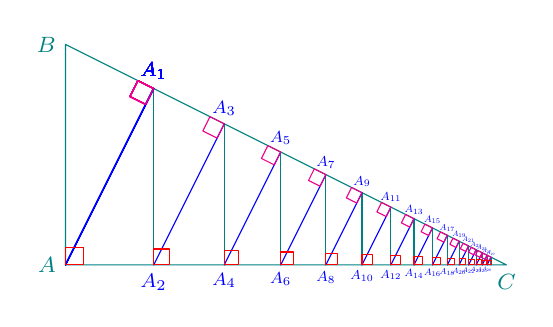
\begin{tikzpicture}[font=\footnotesize, line join=round, line cap=round, >=stealth,teal,scale=0.7]
\def\xx{8}
\def\yy{4}
\pgfmathsetmacro{\gg}{90+atan(\yy/\xx)}
\pgfmathsetmacro{\k}{(\xx)^2/((\xx)^2+(\yy)^2)}
\tikzset{goc/.pic={
\draw(0,0)--(0.25,0)--++(90:0.25)--++(180:0.25)--cycle;
}}
\draw(0,0) node[left]{$A$}--(0,\yy)node[left]{$B$}--(\xx,0)node[below]{$C$}--cycle;
\def\x{0}
\foreach \i in {1,...,15}{
\pgfmathsetmacro{\l}{\xx-(\k)^\i*\xx}
\draw (\l,{(\k)^\i*\yy})coordinate(A\i)--(\l,0)coordinate(B\i);
\global \let \x =\l;
}
\foreach \i in {2,...,15}{
\pgfmathsetmacro{\a}{int(2*\i-1)}
\pgfmathsetmacro{\b}{int(2*\i-2)}
\pgfmathsetmacro{\j}{int(\i-1)}
\draw[blue](A\i)node[above,scale=(0.9)^\i]{$A_{\a}$}pic[yscale=-1,rotate around ={\gg:(A\i)},scale=(0.9)^\i,magenta]{goc}--(B\j)node[below,scale=(0.9)^\j]{$A_{\b}$}pic[yscale=-1,rotate around ={-90:(B\j)},scale=(0.9)^\i,red]{goc};
\draw[blue](A1)node[above,scale=(0.9)]{$A_{1}$}pic[yscale=-1,rotate around ={\gg:(A1)},scale=(0.9)^1,magenta]{goc}--(0,0)node[below]{}pic[yscale=-1,rotate around ={-90:(0,0)},scale=(0.9),red]{goc};
}
\end{tikzpicture}
}
\loigiai{
\begin{itemize}
\item Xét tam giác vuông $ABA_1$ có $AA_1=AB\cdot \sin \alpha = h\sin \alpha$.
\item Xét tam giác vuông $AA_2A_1$ có $\widehat{BAA_1}=\widehat{AA_1A_2}$. \\
Mặt khác $\widehat{BAA_1}+\widehat{ABC}=\widehat{AA_1A_2}+\widehat{A_1AA_2} = 180^\circ \Rightarrow \widehat{A_1AA_2} =\widehat{ABC} =\alpha$.\\
Suy ra
$A_1A_2=AA_1\cdot \sin \alpha = h\sin^2 \alpha$.
\item Lập luận tương tự trên ta có $A_{n-1}A_n= h\sin^n \alpha$.
\end{itemize}
Như vậy $AA_1A_2A_3 \ldots = h\sin \alpha+h\sin^2 \alpha+h\sin^3\alpha+h\sin^4 \alpha \ldots $ là tổng lùi vô hạn của một cấp số nhân có số hạng đầu $u_1=h\sin \alpha$ và công bội là $\sin \alpha$. Do đó $AA_1A_2A_3 \ldots = \dfrac{h\sin \alpha}{1-\sin \alpha}$.
}
\end{ex}

\begin{ex}%[HK1, THPT Nguyễn Thị Minh Khai, 23-24]%[Nguyễn Cường-10-11-HK1]%[1H4C4-6]
Cho hình chóp $S.ABCD$ có đáy $ABCD$ là hình bình hành tâm $O$.
\begin{enumerate}
\item  Gọi $M$ là điểm trên cạnh $SA$ sao cho $\dfrac{SM}{SA}=\dfrac{3}{4}$. Tìm giao tuyến $(d)$ của hai mặt phẳng $(MCD)$ và $(SAB)$
\item  Gọi $I$ là trung điểm của $SD$. Chứng minh rằng: $SB\parallel (IAC)$.
\item  Gọi $J$ là trung điểm của $OA$, $N$ là giao điểm của $(d)$ và $SB$. Chứng minh rằng $(MNJ)\parallel (SCD)$.
\item  Gọi $E$ là giao điểm của $AD$ và $(MNJ), F$ là giao điểm của hai đường thẳng $AI$ và $SE$. Cho biết tam giác $SAD$ là tam giác vuông tại $A$, $SD=a$. Tính $AF$ theo $a$.
\end{enumerate}
\loigiai
{
\begin{center}
\begin{tikzpicture}[scale=1,font=\footnotesize,line join=round,line cap=round,>=stealth]
\path
(0,0) coordinate (A)++(0:4)coordinate(D)++(210:2.5)coordinate(C)++(180:4)coordinate(B)
($(A)!.5!(C)$)coordinate(O)
(A)++(90:3)coordinate(S)
($(S)!3/4!(A)$)coordinate(M)
($(S)!.5!(D)$)coordinate(I)
($(S)!3/4!(B)$)coordinate(N)
($(O)!.5!(A)$)coordinate(J)
($(A)!.25!(D)$)coordinate(E)
($(I)!.25!(D)$)coordinate(G)
(intersection of A--I and S--E)coordinate(F)
;
\draw (S)--(B)--(C)--(D)--(S)
(S)--(C)--(I)
;
\draw[dashed] (E)--(S)--(A)--(D) (C)--(A)--(B)--(D) (A)--(I)--(O)
(M)--(N)--(J)--cycle (J)--(E)--(G)
;
\foreach \x/\g in {A/160,B/-120,C/-90,S/90,D/0,M/180,I/30,O/-90,N/180,J/-90,E/-90,F/180,G/30}
\draw [fill=black] (\x) circle(1pt) +(\g:0.3) node{$\x$};
\end{tikzpicture}
\end{center}
\begin{enumerate}
\item Xét $(MCD)$ và $(SAB)$ có $\heva{&M\in (MCD)\cap (SAB)\\&AB\parallel CD\\&AB\subset (SAB)\\&MN\subset (MCD).}$\\
Do đó, $(SAB)\cap (MCD)=d\parallel AB\parallel CD$ và $d$ đi qua $M$.
\item Do $IO$ là đường trung bình $\triangle SBD$ nên $IO\parallel SB$.\\
Khi đó, $\heva{&SB\not\subset (AIC)\\& SB\parallel OI\\&OI\subset (IAC)}\Rightarrow SB\parallel (IAC)$.
\item Gọi $N=d\cap SB$, ta có $\heva{&MN\not\subset (SCD)\\& MN\parallel CD\\&CD\subset (SCD)}\Rightarrow MN\parallel (SCD)$.\quad\quad (1)\\
Do $\dfrac{AM}{AS}=\dfrac{AJ}{AC}=\dfrac{1}{4}$ nên $MJ\parallel SC$ (định lý Thales).\\
Suy ra $\heva{&MJ\not\subset (SCD)\\& MJ\parallel SC\\&SC\subset (SCD)}\Rightarrow MJ\parallel (SCD)$.\quad\quad (2)\\
Từ $(1)$ và $(2)$, suy ra $(MNJ)\parallel (SCD)$.
\item Ta có $\heva{&I\in (ABCD)\cap (MNJ)\\&MN\parallel AB\\&MN\subset (MNJ)\\&AB\subset (ABCD)}\Rightarrow (ABCD)\cap (MNJ)=d'\parallel AB$ và $d'$ đi qua $J$.\\
Gọi $E=d'\cap AD$, suy ra $E=AD\cap (MNJ)$ đồng thời $\dfrac{AE}{AD}=\dfrac{AI}{AO}=\dfrac{1}{4}$.\\
Gọi $G$ là điểm thuộc $SD$ sao cho $\dfrac{IG}{ID}=\dfrac{1}{4}$.\\
Khi đó, $EG\parallel AI$ và $\dfrac{EG}{AI}=\dfrac{DE}{DA}=\dfrac{3}{4}$.\\
Đồng thời, $\dfrac{FI}{EG}=\dfrac{SI}{SG}=\dfrac{4}{5}$.\\
Từ đó ta có $FI=\dfrac{4}{5}EG=\dfrac{4}{5}\cdot \dfrac{3}{4}AI=\dfrac{3}{5}AI$.\\
Do đó, $AF=\dfrac{2}{5}AI=\dfrac{2}{5}\cdot \dfrac{1}{2}SD=\dfrac{a}{5}$.
\end{enumerate}
}
\end{ex}

\Closesolutionfile{ans}
